\documentclass[10pt]{article}
\usepackage[utf8]{inputenc}
\usepackage[T1]{fontenc}
\usepackage{amsmath}
\usepackage{amsfonts}
\usepackage{amssymb}
\usepackage[version=4]{mhchem}
\usepackage{stmaryrd}
\usepackage{graphicx}
\usepackage[export]{adjustbox}
\graphicspath{ {./images/} }
\usepackage{bbold}

\begin{document}
\section*{Math 141 Tutorial 2 Solutions}
\section*{Main problems}
\begin{enumerate}
  \item Using the summation formulas seen in class, provide a closed form for the following summations in terms of $n$.\\
(a) $\sum_{i=0}^{n}(i+1)$\\
(d) $\sum_{i=0}^{n}(i-2)^{2}$\\
(b) $\sum_{i=2}^{n}(2 i+n)$\\
(e) $\sum_{i=-n}^{0}-i^{3}$\\
(c) $\sum_{i=-1}^{n}(i+2)^{2}$\\
(f) $\sum_{i=-n}^{n}\left(i^{3}+3 i^{2} n+3 i n^{2}+n^{3}\right)$
\end{enumerate}

Solutions:\\
(a) By linearity, we have

$$
\begin{aligned}
\sum_{i=0}^{n}(i+1)=\sum_{i=0}^{n} i+\sum_{i=0}^{n} 1 & =\sum_{i=1}^{n} i+(n+1) \\
& =\frac{n(n+1)}{2}+(n+1) \\
& =\frac{n(n+1)+2(n+1)}{2} \\
& =\frac{n^{2}+3 n+2}{2}
\end{aligned}
$$

(b) We can proceed similarly here, but we must be a little careful when applying the identity $\sum_{i=1}^{n} i=\frac{n(n+1)}{2}$ because our sum begins at $i=2$. To circumvent this issue, we proceed as follows (adding and subtracting 1 in order to introduce the "missing term")

$$
\sum_{i=2}^{n}(2 i+n)=\sum_{i=2}^{n} 2 i+\sum_{i=2}^{n} n=2 \sum_{i=2}^{n} i+\underbrace{\sum_{i=2}^{n} 1}_{\substack{(n-1) \\ \text { terms }}}
$$

$$
\begin{aligned}
& =2[\underbrace{-1+1}_{=0}+\sum_{i=2}^{n} i]+n(n-1) \\
& =2\left[-1+\sum_{i=1}^{n} i\right]+n(n-1) \\
& =2\left[-1+\frac{n(n+1)}{2}\right]+n(n-1) \\
& =2\left[\frac{n^{2}+n-2}{2}\right]+n(n-1) \\
& =n^{2}+n-2+n^{2}-n \\
& =2 n^{2}-2
\end{aligned}
$$

(c) We have

$$
\begin{aligned}
\sum_{i=-1}^{n}(i+2)^{2} & =\left[(-1+2)^{2}+(0+2)^{2}+\cdots+(n-1+2)^{2}+(n+2)^{2}\right] \\
& =\left[(1)^{2}+(2)^{2}+\cdots+(n+1)^{2}+(n+2)^{2}\right] \\
& =\sum_{j=1}^{n+2} j^{2} \\
& =\frac{(n+2)((n+2)+1)(2(n+2)+1)}{6} \\
& =\frac{(n+2)(n+3)(2 n+5)}{6}
\end{aligned}
$$

(d) We write

$$
\begin{aligned}
\sum_{i=0}^{n}(i-2)^{2} & =(-2)^{2}+(-1)^{2}+0^{2}+1^{2}+2^{2}+\cdots+(n-1-2)^{2}+(n-2)^{2} \\
& =5+1^{2}+2^{2}+\cdots+(n-1-2)^{2}+(n-2)^{2} \\
& =5+\sum_{j=1}^{n-2} j^{2} \\
& =5+\frac{(2(n-2)+1)(n-2)(n-1)}{6} \\
& =\frac{30+2 n^{3}-9 n^{2}+13 n-6}{6} \\
& =\frac{2 n^{3}-9 n^{2}+13 n+24}{6}
\end{aligned}
$$

(e) Simply note that

$$
\sum_{i=-n}^{1}-i^{3}=-\sum_{i=-n}^{1} i^{3}=-\left((-n)^{3}+(-(n-1))^{3}+\cdots+(-2)^{3}+(-1)^{3}\right)
$$

Page 2

$$
\begin{aligned}
& =-\left(-n^{3}-(n-1)^{3}-\cdots-2^{3}-1^{3}\right) \\
& =\left(n^{3}+(n-1)^{3}+\cdots+2^{3}+1^{3}\right) \\
& =\left(1^{3}+2^{3}+\cdots+n^{3}\right) \\
& =\sum_{j=1}^{n} j^{3} \\
& =\frac{n^{2}(n+1)^{2}}{4}
\end{aligned}
$$

(f) Notice that $i^{3}+3 i^{2} n+3 i n^{2}+n^{3}=(i+n)^{3}$, as can be seen by expanding the latter expression. Hence, we see that

$$
\begin{aligned}
\sum_{i=-n}^{n} & \left(i^{3}+3 i^{2} n+3 i n^{2}+n^{3}\right) \\
& =\sum_{i=-n}^{n}(n+i)^{3} \\
& =(n-n)^{3}+(n+(-n+1))^{3}+\cdots+(n+0)^{3}+(n+1)^{3}+\cdots+(n+(n-1))^{3}+(n+n)^{3} \\
& =0+1+\cdots+n^{3}+(n+1)^{3}+\cdots+(2 n-1)^{3}+(2 n)^{3} \\
& =\sum_{j=1}^{2 n} j^{3} \\
& =\frac{(2 n)^{2}(2 n+1)^{2}}{4} \\
& =(2 n+1)^{2} n^{2}
\end{aligned}
$$

\begin{enumerate}
  \setcounter{enumi}{1}
  \item Evaluate the definite integrals by either taking the limit of (left or right) Riemann sums or interpreting the integral as an area.\\
(a) $\int_{0}^{2} 2 x \mathrm{~d} x$\\
(d) $\int_{1}^{5}\left(x^{2}+2 x\right) \mathrm{d} x$\\
(b) $\int_{1}^{4}(3-x) \mathrm{d} x$\\
(e) $\int_{0}^{3} x^{3} \mathrm{~d} x$\\
(c) $\int_{0}^{2}\left(2 x^{2}+1\right) \mathrm{d} x$\\
(f) $\int_{-2}^{2}|2 x| \mathrm{d} x$
\end{enumerate}

Solutions:\\
(a) We can interpret this integral as the area of the following triangle:\\
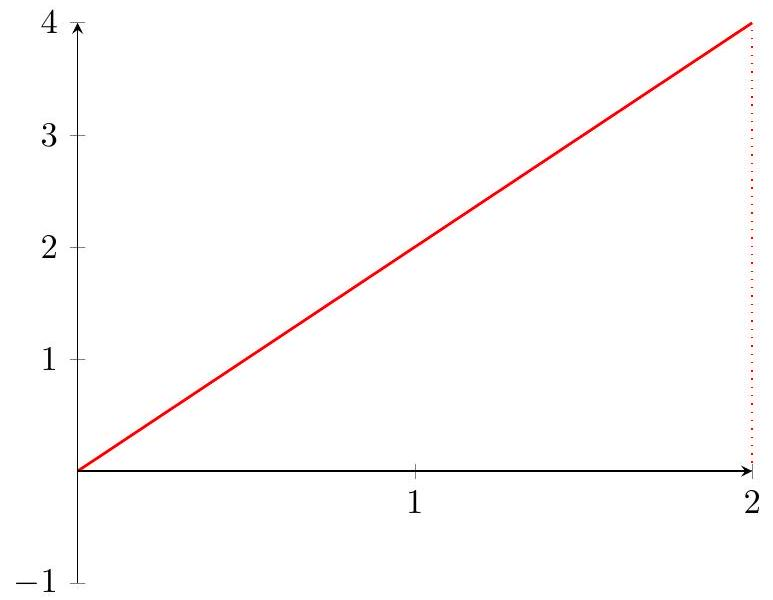
\includegraphics[max width=\textwidth, center]{2024_12_27_c77fac7b45ac922a81d8g-04}

Geometrically, we see that the triangle has base length 2 and height 4, thus we have

$$
\int_{0}^{2} 2 x \mathrm{~d} x=\frac{2 \cdot 4}{2}=4
$$

(b) Similarly, we'll calculate the value of the integral as an area:\\
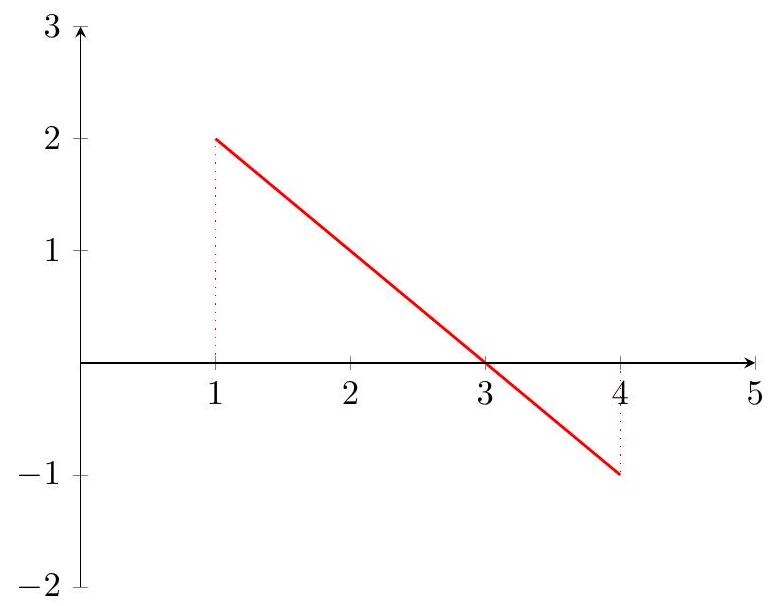
\includegraphics[max width=\textwidth, center]{2024_12_27_c77fac7b45ac922a81d8g-05}

Notice that we have two triangles - the first has base length 2 and height 2 while the second has base length 1 and height 1 . Since the second triangle is below the x-axis, we'll consider this area to be "negative" (we can pretend that the triangle has "height -1 "), so we get

$$
\int_{1}^{4}(3-x) \mathrm{d} x=\frac{3 \cdot 2}{2}+\frac{1 \cdot(-1)}{2}=\frac{5}{2}
$$

(c) We begin by writing out the right Riemann sum with $n$-subintervals. The interval $[0,2]$ has length 2, so the width of the rectangles in the Riemann sum will be $\Delta x=2 / n$. Then the nodes/tag points are given by

$$
x_{i}^{*}=0+i \Delta x=\frac{2 i}{n}, \quad(i=1, \ldots, n)
$$

Then the right Riemann sum for $2 x^{2}+1$ on $[0,2]$ with $n$-subintervals is

$$
\begin{aligned}
R_{n}=\sum_{i=1}^{n}\left(2\left(x_{i}^{*}\right)^{2}+1\right) \Delta x & =\sum_{i=1}^{n}\left[2\left(\frac{2 i}{n}\right)^{2}+1\right] \frac{2}{n} \\
& =\sum_{i=1}^{n}\left[\frac{8 i^{2}}{n^{2}}+1\right] \frac{2}{n} \\
& =\frac{2}{n}\left[\frac{8}{n^{2}} \sum_{i=1}^{n} i^{2}+\sum_{i=1}^{n} 1\right] \\
& =\frac{2}{n}\left[\frac{8}{n^{2}} \frac{n(n+1)(2 n+1)}{6}+n\right], \\
& =\frac{8}{3} \frac{(n+1)(2 n+1)}{n^{2}}+2 .
\end{aligned}
$$

Since the given function is continuous on $[0,2]$, it is integrable there. Consequently, the Riemann sums $R_{n}$ converge to the value $\int_{0}^{2}\left(2 x^{2}+1\right) \mathrm{d} x$ as $n \rightarrow \infty$. That is, we have

$$
\int_{0}^{2}\left(2 x^{2}+1\right) \mathrm{d} x=\lim _{n \rightarrow \infty} R_{n}=\lim _{n \rightarrow \infty} \frac{8}{3} \frac{(n+1)(2 n+1)}{n^{2}}+2
$$

$$
\begin{aligned}
& =\frac{16}{3}+2 \\
& =\frac{22}{3}
\end{aligned}
$$

(d) Since our interval $[1,5]$ has length 4 , the width of the rectangles will be $\Delta x=4 / n$. Then, the nodes (or tag points) are given by

$$
x_{i}^{*}=1+i \Delta x=1+\frac{4 i}{n}, \quad(i=1, \ldots, n)
$$

Thus, the right Riemann sum for $x^{2}+2 x$ on $[1,5]$ with $n$-subintervals is

$$
\begin{aligned}
R_{n}=\sum_{i=1}^{n}\left(\left(x_{i}^{*}\right)^{2}+2 x_{i}^{*}\right) \Delta x & =\sum_{i=1}^{n}\left[\left(1+\frac{4 i}{n}\right)^{2}+2\left(1+\frac{4 i}{n}\right)\right] \frac{4}{n} \\
& =\sum_{i=1}^{n}\left[1+\frac{8 i}{n}+\frac{16 i^{2}}{n^{2}}+2+\frac{8 i}{n}\right] \frac{4}{n} \\
& =\frac{4}{n} \sum_{i=1}^{n}\left[3+\frac{16 i}{n}+\frac{16 i^{2}}{n^{2}}\right] \\
& =\frac{4}{n}\left[\sum_{i=1}^{n} 3+\frac{16}{n} \sum_{i=1}^{n} i+\frac{16}{n^{2}} \sum_{i=1}^{n} i^{2}\right] \\
& =\frac{4}{n}\left[3 n+\frac{16}{n} \cdot \frac{n(n+1)}{2}+\frac{16}{n^{2}} \cdot \frac{n(n+1)(2 n+1)}{6}\right] \\
& =\frac{4}{n}\left[3 n+8(n+1)+\frac{8(n+1)(2 n+1)}{3 n}\right] \\
& =4\left(11+\frac{1}{n}+\frac{8(n+1)(2 n+1)}{3 n^{2}}\right) \\
& =4\left(11+\frac{1}{n}+\frac{16 n^{2}+24 n+8}{3 n^{2}}\right)
\end{aligned}
$$

Taking the limit, it follows that

$$
\begin{aligned}
\int_{1}^{5}\left(x^{2}+2 x\right) \mathrm{d} x=\lim _{n \rightarrow \infty} R_{n} & =\lim _{n \rightarrow \infty} 4\left(11+\frac{1}{n}+\frac{16 n^{2}+24 n+8}{3 n^{2}}\right) \\
& =4\left(11+\frac{16}{3}\right) \\
& =\frac{196}{3}
\end{aligned}
$$

(e) We proceed as in the previous problem with right Riemann sums. Since $f(x)=x^{3}$ is continuous on [0,3], it is Riemann integrable there and, furthermore, the right Riemann sums must converge to $\int_{0}^{3} x^{3} \mathrm{~d} x$ as $n \rightarrow \infty$. Computing the right Riemann sum for $f(x)=x^{3}$ on $[0,3]$ gives $\Delta x=3 / n$ and

$$
R_{n}(f)=\sum_{i=1}^{n}\left(x_{i}^{*}\right)^{3} \Delta x=\sum_{i=1}^{n}\left(0+i \frac{3}{n}\right)^{3} \frac{3}{n}
$$

$$
\begin{aligned}
& =\sum_{i=1}^{n} \frac{3^{4} i^{3}}{n^{4}} \\
& =\frac{81}{n^{4}} \sum_{i=1}^{n} i^{3} \\
& =\frac{81}{n^{4}} \cdot \frac{n^{2}(n+1)^{2}}{4} \\
& =\frac{81\left(n^{4}+2 n^{3}+2 n\right)}{4}
\end{aligned}
$$

Taking the limit as $n \rightarrow \infty$, we infer that

$$
\int_{0}^{3} x^{3} \mathrm{~d} x=\lim _{n \rightarrow \infty} R_{n}(f)=\lim _{n \rightarrow \infty} \frac{81\left(n^{4}+2 n^{3}+2 n\right)}{4}=\frac{81}{4} .
$$

(f) We now examine $\int_{-2}^{2}|2 x| \mathrm{d} x$. To deal with the absolute value that appears, we will break the integral into a sum of two integrals, on which $|2 x|$ is either positive or negative. This is done in the following way:

$$
\int_{-2}^{2}|2 x| \mathrm{d} x=\int_{-2}^{0}-(2 x) \mathrm{d} x+\int_{0}^{2}(2 x) \mathrm{d} x=\int_{0}^{2} 2 x \mathrm{~d} x-\int_{-2}^{0} 2 x \mathrm{~d} x .
$$

Clearly, these two integrals should each be easier to evaluate than the original integral we started with. Since $2 x$ is Riemann integrable by continuity, the integral $\int_{0}^{2} 2 x \mathrm{~d} x$ is the limit of the right Riemann sums as $n \rightarrow \infty$, i.e.

$$
\begin{aligned}
\int_{0}^{2} 2 x \mathrm{~d} x & =\lim _{n \rightarrow \infty} \sum_{i=1}^{n} 2\left(\frac{2 i}{n}\right) \frac{2}{n} \\
& =\lim _{n \rightarrow \infty} \frac{8}{n^{2}} \sum_{i=1}^{n} i \\
& =\lim _{n \rightarrow \infty} \frac{8}{n^{2}} \cdot \frac{n(n+1)}{2} \\
& =\lim _{n \rightarrow \infty} \frac{4 n^{2}+4 n}{n^{2}} \\
& =4
\end{aligned}
$$

In order to compute $\int_{-2}^{0} 2 x \mathrm{~d} x$, we will also make use of right Riemann sums. Here, we also have $\Delta x=\frac{0-(-2)}{n}=\frac{2}{n}$. However, the nodes are instead given by

$$
x_{i}^{*}=-2+\frac{2 i}{n}, \quad(i=1, \ldots, n)
$$

Thus,

$$
\int_{-2}^{0} 2 x \mathrm{~d} x=\lim _{n \rightarrow \infty} \sum_{i=1}^{n} 2\left(-2+\frac{2 i}{n}\right) \frac{2}{n}
$$

$$
\begin{aligned}
& =\lim _{n \rightarrow \infty} \frac{8}{n} \sum_{i=1}^{n}\left(-1+\frac{i}{n}\right) \\
& =\lim _{n \rightarrow \infty}\left(\frac{8}{n} \sum_{i=1}^{n}(-1)+\frac{8}{n^{2}} \sum_{i=1}^{n} i\right) \\
& =\lim _{n \rightarrow \infty}\left(\frac{8}{n} \cdot(-n)+\frac{8}{n^{2}} \cdot \frac{n(n+1)}{2}\right) \\
& =\lim _{n \rightarrow \infty}\left(-8+\frac{4 n^{2}+4 n}{n^{2}}\right) \\
& =-4
\end{aligned}
$$

Now, putting together all our work gives:

$$
\int_{-2}^{2}|2 x| \mathrm{d} x=\int_{0}^{2} 2 x \mathrm{~d} x-\int_{-2}^{0} 2 x \mathrm{~d} x=4-(-4)=8
$$

Page 8\\
3. Suppose that $f, g:[a, b] \rightarrow \mathbb{R}$ are continuous functions and let $k \in \mathbb{R}$ be a constant. By using the corresponding properties for summations, prove the following\\
(a) $\int_{a}^{b}(k f(x)) \mathrm{d} x=k \int_{a}^{b} f(x) \mathrm{d} x$\\
(b) $\int_{a}^{b}(f(x)+g(x)) \mathrm{d} x=\int_{a}^{b} f(x) \mathrm{d} x+\int_{a}^{b} g(x) \mathrm{d} x$

Solutions:\\
(a) Since $f$ is continuous on the interval $[a, b]$, it must be Riemann integrable on $[a, b]$. Therefore, if we let $R_{n}(f)$ denote the right Riemann sum of $f$ with $n$-subintervals, we have


\begin{equation*}
\lim _{n \rightarrow \infty} R_{n}(f)=\int_{a}^{b} f(x) \mathrm{d} x \tag{1}
\end{equation*}


That is, the Riemann sums of $f$ converge to $\int_{a}^{b} f \mathrm{~d} x$ as $n \rightarrow \infty$. Similarly, because $f$ is continuous on $[a, b]$ and $k \in \mathbb{R}$ is a constant, the function $k f(x)$ is continuous and integrable on $[a, b]$. By the same logic, the right Riemann sum of $k f$ will converge to $\int_{a}^{b} k f(x) \mathrm{d} x$ as $n \rightarrow \infty$, i.e.


\begin{equation*}
\lim _{n \rightarrow \infty} R_{n}(k f)=\int_{a}^{b} k f(x) \mathrm{d} x \tag{2}
\end{equation*}


But then, because we can pull constants out of finite sums, we obtain

$$
\begin{aligned}
\int_{a}^{b} k f(x) \mathrm{d} x=\lim _{n \rightarrow \infty} R_{n}(k f) & =\lim _{n \rightarrow \infty} \sum_{i=1}^{n}\left(k f\left(x_{i}^{*}\right)\right) \Delta x \\
& =\sum_{i=1}^{n} k f\left(x_{i}^{*}\right) \Delta x \\
& =k \sum_{i=1}^{n} f\left(x_{i}^{*}\right) \Delta x \\
& =k R_{n}(f) .
\end{aligned}
$$

Combining this with (1)-(2), this implies that

$$
\begin{aligned}
\int_{a}^{b} k f(x) \mathrm{d} x=\lim _{n \rightarrow \infty} R_{n}(k f) & =\lim _{n \rightarrow \infty}\left(k R_{n}(f)\right) \\
& =k \lim _{n \rightarrow \infty} R_{n}(f) \\
& =k \int_{a}^{b} f(x) \mathrm{d} x
\end{aligned}
$$

(b) Since $f$ and $g$ are continuous on the interval $[a, b]$, their sum $f+g$ is also continuous on $[a, b]$. Especially, the functions $f, g$ and $f+g$ are Riemann integrable on $[a, b]$. Furthermore, as in the previous exercise, this means that

$$
\lim _{n \rightarrow \infty} R_{n}(f)=\int_{a}^{b} f(x) \mathrm{d} x
$$

$$
\begin{aligned}
\lim _{n \rightarrow \infty} R_{n}(g) & =\int_{a}^{b} g(x) \mathrm{d} x \\
\lim _{n \rightarrow \infty} R_{n}(f+g) & =\int_{a}^{b}(f(x)+g(x)) \mathrm{d} x
\end{aligned}
$$

where $R_{n}(\cdot)$ once again denotes the right Riemann sum of a function. However, the Riemann sums satisfy

$$
\begin{aligned}
R_{n}(f+g)=\sum_{i=1}^{n}(f+g)\left(x_{i}^{*}\right) \Delta x & =\sum_{i=1}^{n}\left(f\left(x_{i}^{*}\right)+g\left(x_{i}^{*}\right)\right) \Delta x \\
& =\sum_{i=1}^{n} f\left(x_{i}^{*}\right) \Delta x+\sum_{i=1}^{n} g\left(x_{i}^{*}\right) \Delta x \\
& =R_{n}(f)+R_{n}(g) .
\end{aligned}
$$

Taking the limit as $n \rightarrow \infty$ and applying the limit laws from Math 140, we infer that

$$
\begin{aligned}
\int_{a}^{b}(f(x)+g(x)) \mathrm{d} x & =\lim _{n \rightarrow \infty} R_{n}(f+g) \\
& =\lim _{n \rightarrow \infty}\left(R_{n}(f)+R_{n}(g)\right) \\
& =\lim _{n \rightarrow \infty} R_{n}(f)+\lim _{n \rightarrow \infty} R_{n}(g) \\
& =\int_{a}^{b} f(x) \mathrm{d} x+\int_{a}^{b} g(x) \mathrm{d} x .
\end{aligned}
$$

\section*{Challenge problems}
\begin{enumerate}
  \setcounter{enumi}{3}
  \item Using Riemann sums, show that
\end{enumerate}

$$
\int_{a(x)}^{b(x)} t \mathrm{~d} t=\frac{(b(x))^{2}-(a(x))^{2}}{2}
$$

\begin{enumerate}
  \setcounter{enumi}{4}
  \item What do you expect the value of
\end{enumerate}

$$
\int_{-\pi / 2}^{3 \pi / 2} \cos x \mathrm{~d} x
$$

to be? Hint: use symmetry.\\
6. Let $f(x)=x^{2}$.\\
(a) Using Riemann sums, determine the function

$$
F(x)=\int_{0}^{x} f(t) \mathrm{d} t
$$

(b) Determine the derivative $F^{\prime}(x)$ of $F(x)$. How does this function relate to $f$ ?


\end{document}